% !TEX root = ../main.tex

\chapter{Appendix} % Main appendix title
\label{ch:appendix}

\section{Generated C++ code for books\_200M with 32-bit keys}
\label{sect:appendix:books_200M_uint32_0}

\subsection{Header file (L0 parameters)}

\begin{C++}
namespace books_200M_uint32_0 {
  const double L0_PARAMETER0 = 0.0;
  const double L0_PARAMETER1 = 0.0;
  const double L0_PARAMETER2 = 0.003906249768078851;
  const double L0_PARAMETER3 = 0.0;
  char* L1_PARAMETERS;
}\end{C++}

\subsection{Code file (Lookup code)}

\begin{C++}
#include "books_200M_uint32_0_data.h"
#include <math.h>
#include <cmath>
#include <fstream>
#include <filesystem>
#include <iostream>
namespace books_200M_uint32_0 {
bool load(char const* dataPath) {
  {
    std::ifstream infile(std::filesystem::path(dataPath) / "books_200M_uint32_0_L1_PARAMETERS", std::ios::in | std::ios::binary);
    if (!infile.good()) return false;
    L1_PARAMETERS = (char*) malloc(402653184);
    if (L1_PARAMETERS == NULL) return false;
    infile.read((char*)L1_PARAMETERS, 402653184);
    if (!infile.good()) return false;
  }
  return true;
}
void cleanup() {
  free(L1_PARAMETERS);
}

inline double linear(double alpha, double beta, double inp) {
  return std::fma(beta, inp, alpha);
}

inline double cubic(double a, double b, double c, double d, double x) {
  auto v1 = std::fma(a, x, b);
  auto v2 = std::fma(v1, x, c);
  auto v3 = std::fma(v2, x, d);
  return v3;
}

inline size_t FCLAMP(double inp, double bound) {
  if (inp < 0.0) return 0;
  return (inp > bound ? bound : (size_t)inp);
}

uint64_t lookup(uint64_t key, size_t* err) {
  double fpred;
  size_t modelIndex;
  fpred = cubic(L0_PARAMETER0, L0_PARAMETER1, L0_PARAMETER2, L0_PARAMETER3, (double)key);
  modelIndex = (uint64_t) fpred;
  fpred = linear(*((double*) (L1_PARAMETERS + (modelIndex * 24) + 0)), *((double*) (L1_PARAMETERS + (modelIndex * 24) + 8)), (double)key);
  *err = *((uint64_t*) (L1_PARAMETERS + (modelIndex * 24) + 16));

  return FCLAMP(fpred, 200000000.0 - 1.0);
}
}\end{C++}


\section{FMA operation in P4}
\label{sect:appendix:fma}

\subsection{Addition}
\label{sect:appendix:floating_addition}

\begin{P4}
action floating_add(in double_t first, in double_t second, out overflow128_t result) {
  bool first_bigger = first.exponent == second.exponent ? first.mantissa > second.mantissa : first.exponent > second.exponent;
  uint64_t first_mantissa = ((uint64_t) first.mantissa) | HIDDEN_BIT;
  uint64_t second_mantissa = ((uint64_t) second.mantissa) | HIDDEN_BIT;

  if ((first.exponent == 0 && first.mantissa == 0) || (second.exponent == 0 && second.mantissa == 0)) {
    if (first.exponent == 0 && first.mantissa == 0) {
      result = { second.sign, second.exponent, (bit<128>) second_mantissa }; // first zero, return second
    } else {
      result = { first.sign, first.exponent, (bit<128>) first_mantissa }; // second zero, return first
    }
    return;
  }

  exponent_t exponent_difference = first_bigger ? (first.exponent - second.exponent) : (second.exponent - first.exponent);
  uint64_t bigger_mantissa = first_bigger ? first_mantissa : second_mantissa;
  uint64_t smaller_mantissa = first_bigger ? second_mantissa : first_mantissa;
  smaller_mantissa = smaller_mantissa >> ((bit<8>) exponent_difference);

  result.sign = first_bigger ? first.sign : second.sign;
  result.exponent = first_bigger ? first.exponent : second.exponent;
  if (first.sign != second.sign) { // inputs have different sign, this is a subtraction
    result.mantissa = (bit<128>) (bigger_mantissa - smaller_mantissa);
  } else { // both numbers have the same sign, regular addition
    result.mantissa = (bit<128>) (bigger_mantissa + smaller_mantissa);
  }
}

control FloatingAdder(in double_t first, in double_t second, out double_t result) {
  FloatingNormalizer() normalizer;

  overflow128_t temp;
  apply {
    floating_add(first, second, temp);
    normalizer.apply(temp);
    result = { temp.sign, temp.exponent, (mantissa_t) temp.mantissa };
  }
}\end{P4}

\subsection{Multiplication}
\label{sect:appendix:floating_multiplication}

\begin{P4}
action floating_multiply(in double_t first, in double_t second, out overflow128_t result) {
  if ((first.exponent == 0 && first.mantissa == 0) || (second.exponent == 0 && second.mantissa == 0)) {
    result = { first.sign ^ second.sign, 0, 0 }; return;
  }

  result.sign = first.sign ^ second.sign; // ^ = xor
  result.exponent = (first.exponent - EXPONENT_BIAS) + (second.exponent - EXPONENT_BIAS) + EXPONENT_BIAS;

  bit<128> first_mantissa = ((bit<128>) first.mantissa) | (bit<128>) HIDDEN_BIT;
  bit<128> second_mantissa = ((bit<128>) second.mantissa) | (bit<128>) HIDDEN_BIT;

  result.mantissa = (first_mantissa * second_mantissa) >> 52;
}

control FloatingMultiplier(in double_t first, in double_t second, out double_t result) {
  FloatingNormalizer() normalizer;

  overflow128_t temp;
  apply {
    floating_multiply(first, second, temp);
    normalizer.apply(temp);
    result = { temp.sign, temp.exponent, (mantissa_t) temp.mantissa };
  }
}\end{P4}

\subsection{Normalization}
\label{sect:appendix:floating_normalization}

\begin{P4}
control FloatingNormalizer(inout overflow128_t overflow) {
  action floating_shift_left(inout overflow128_t result, bit<8> amount) {
    result.mantissa = result.mantissa << amount;
    result.exponent = result.exponent - (exponent_t) amount;
  }

  action floating_shift_right(inout overflow128_t result, bit<8> amount) {
    result.mantissa = result.mantissa >> amount;
    result.exponent = result.exponent + (exponent_t) amount;
  }

  table floating_normalize {
    key = {
      overflow.mantissa: ternary;
    }
    actions = {
      floating_shift_left(overflow);
      floating_shift_right(overflow);
      NoAction;
    }
    const default_action = NoAction();
    const entries =  { // value to match against &&& bit mask
      0b1000...0 &&& 0b100...0: floating_shift_right(overflow, 75);
      0b0100...0 &&& 0b110...0: floating_shift_right(overflow, 74);
      0b0010...0 &&& 0b111...0: floating_shift_right(overflow, 73);
      // ...
      // the mask where the first significant bit is at pos 53 needs no action
      // ...
      0b0...0100 &&& 0b1...100: floating_shift_left(overflow, 50);
      0b0...0010 &&& 0b1...110: floating_shift_left(overflow, 51);
      0b0...0001 &&& 0b1...111: floating_shift_left(overflow, 52);
    }
  }

  apply {
      floating_normalize.apply();
  }
}\end{P4}

\subsection{FMA}
\label{sect:appendix:fma}

\begin{P4}
control FloatingFusedMultiplyAdd(in double_t x, in double_t y, in double_t z, out double_t result) {
  FloatingAdder() adder_instance;
  FloatingMultiplier() multiplier_instance;

  apply {
    multiplier_instance.apply(x, y, result);
    adder_instance.apply(result, z, result);
  }
}\end{P4}

\section{Loading model parameters}

\subsection{Data plane RMI table declaration in P4}
\label{sect:appendix:rmi_table}

\begin{P4}
control ModelLookup(in uint64_t model_index, out double_t first_l1, out double_t second_l1, out uint64_t err) {

  action assign_variables(sign_t first_sign, exponent_t first_exponent, mantissa_t first_mantissa,
                          sign_t second_sign, exponent_t second_exponent, mantissa_t second_mantissa,
                          uint64_t err_val) {
      first_l1 = { first_sign, first_exponent, first_mantissa };
      second_l1 = { second_sign, second_exponent, second_mantissa };
      err = err_val;
  }

  table model_lookup {
      key = {
          model_index: exact;
      }
      actions = {
          assign_variables;
          NoAction;
      }
      const default_action = assign_variables(0, 0, 0, 0, 0, 0, 0);
      const size = 550000; // depends on model parameter size
  }
  apply {
      assign_variables(0, 0, 0, 0, 0, 0, 0);
      model_lookup.apply();
  }
}\end{P4}

\subsection{Control plane batch sending of model parameters in Python}
\label{sect:appendix:sending_params}

\begin{python}
BATCH_SIZE = 2048

SIGN_MASK = 0x8000000000000000
EXPONENT_MASK = 0x7FF0000000000000
MANTISSA_MASK = 0x000FFFFFFFFFFFFF

def writeL1Parameters(p4info_helper, switch):
  if not os.path.exists('path/to/layer_parameters'): print('Parameters file not found!'); return
  model_index = 0
  with open('path/to/layer_parameters', 'rb') as file:
    bytes = file.read(24 * BATCH_SIZE)
    while bytes:
      entries_batch = []
      for index in range(0, BATCH_SIZE):
        model_bytes = bytes[(24 * index):(24 * (index + 1))]
        first_l1 = int.from_bytes(model_bytes[0:8], byteorder='little')
        second_l1 = int.from_bytes(model_bytes[8:16], byteorder='little')
        third_l1 = int.from_bytes(model_bytes[16:24], byteorder='little')

        table_entry = p4info_helper.buildTableEntry(
          table_name='LearnedIngress.lookup_instance.l1_lookup.l1_model_lookup',
          match_fields={ 'model_index': model_index },
          action_name='LearnedIngress.lookup_instance.l1_lookup.assign_variables',
          action_params={
            'first_l1_sign': (first_l1 & SIGN_MASK) >> 63,
            'first_l1_exponent': (first_l1 & EXPONENT_MASK) >> 52,
            'first_l1_mantissa': first_l1 & MANTISSA_MASK,
            'second_l1_sign': (second_l1 & SIGN_MASK) >> 63,
            'second_l1_exponent': (second_l1 & EXPONENT_MASK) >> 52,
            'second_l1_mantissa': second_l1 & MANTISSA_MASK,
            'third_l1_input': third_l1
          })
        entries_batch.append(table_entry)
        model_index += 1

      switch.WriteTableEntries(entries_batch)
      bytes = file.read(24 * BATCH_SIZE)\end{python}

\section{RMI lookup fuction in P4}
\label{sect:appendix:rmi_lookup}

\begin{P4}
control LearnedLookup(in double_t input_key, out uint64_t guess, out uint64_t guess_err) {
  ModelLookup() lookup_instance;
  LearnedCubic() cubic_instance;
  LearnedLinear() linear_instance;

  double_t fpred;
  uint64_t model_index;
  double_t first_l1; double_t second_l1;

  apply {
    // 1. using static L0 parameters as input for the first cubic model layer
    cubic_instance.apply({ 0, 0, 0 }, { 0, 0, 0 }, { 0, 1014, 4503599092596736 }, { 0, 0, 0 }, input_key, fpred);
    double_to_int(fpred, model_index);

    lookup_instance.apply(model_index, first_l1, second_l1, guess_err); // 2. retrieving L1 parameters

    // 3. using retrieved L1 parameters as input for second linear model layer
    linear_instance.apply(first_l1, second_l1, input_key, fpred);
    double_to_int(fpred, guess);

    f_clamp(fpred, 0xbebc1ff, guess);
  }
}\end{P4}

\newpage % ugly, but otherwise latex does not place section title correctly

\section{Experiment results using cold caches and memory fencing}
\label{sect:appendix:measurements}

\captionsetup[figure]{skip=10pt} % move caption down
\begin{figure}[!htb]
  \centering
  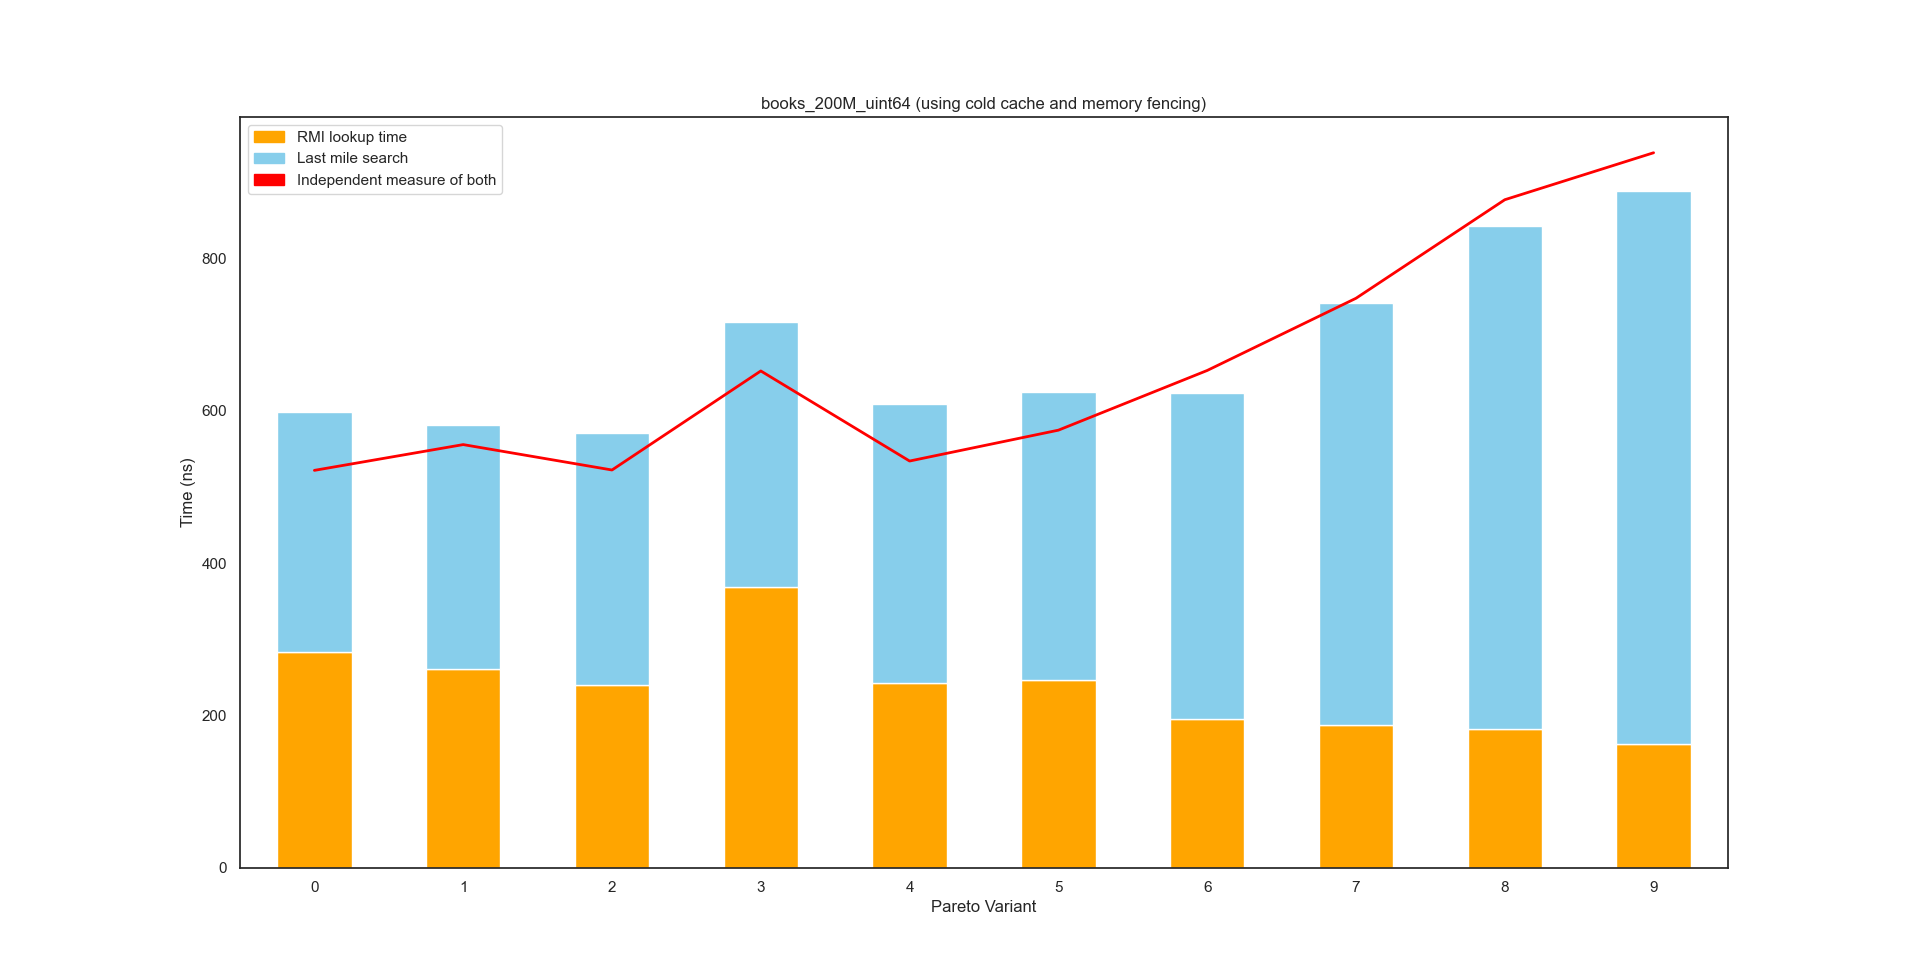
\includegraphics[width=1\textwidth]{measurements/books_200M_uint64}
  \caption*{
    Running the SOSD benchmark on the \emph{books\_200M\_uint64} dataset \emph{using} cold caches and memory fencing, differentiating between pure lookup time and last mile search time.
  }
\end{figure}

\begin{figure}[!htb]
  \centering
  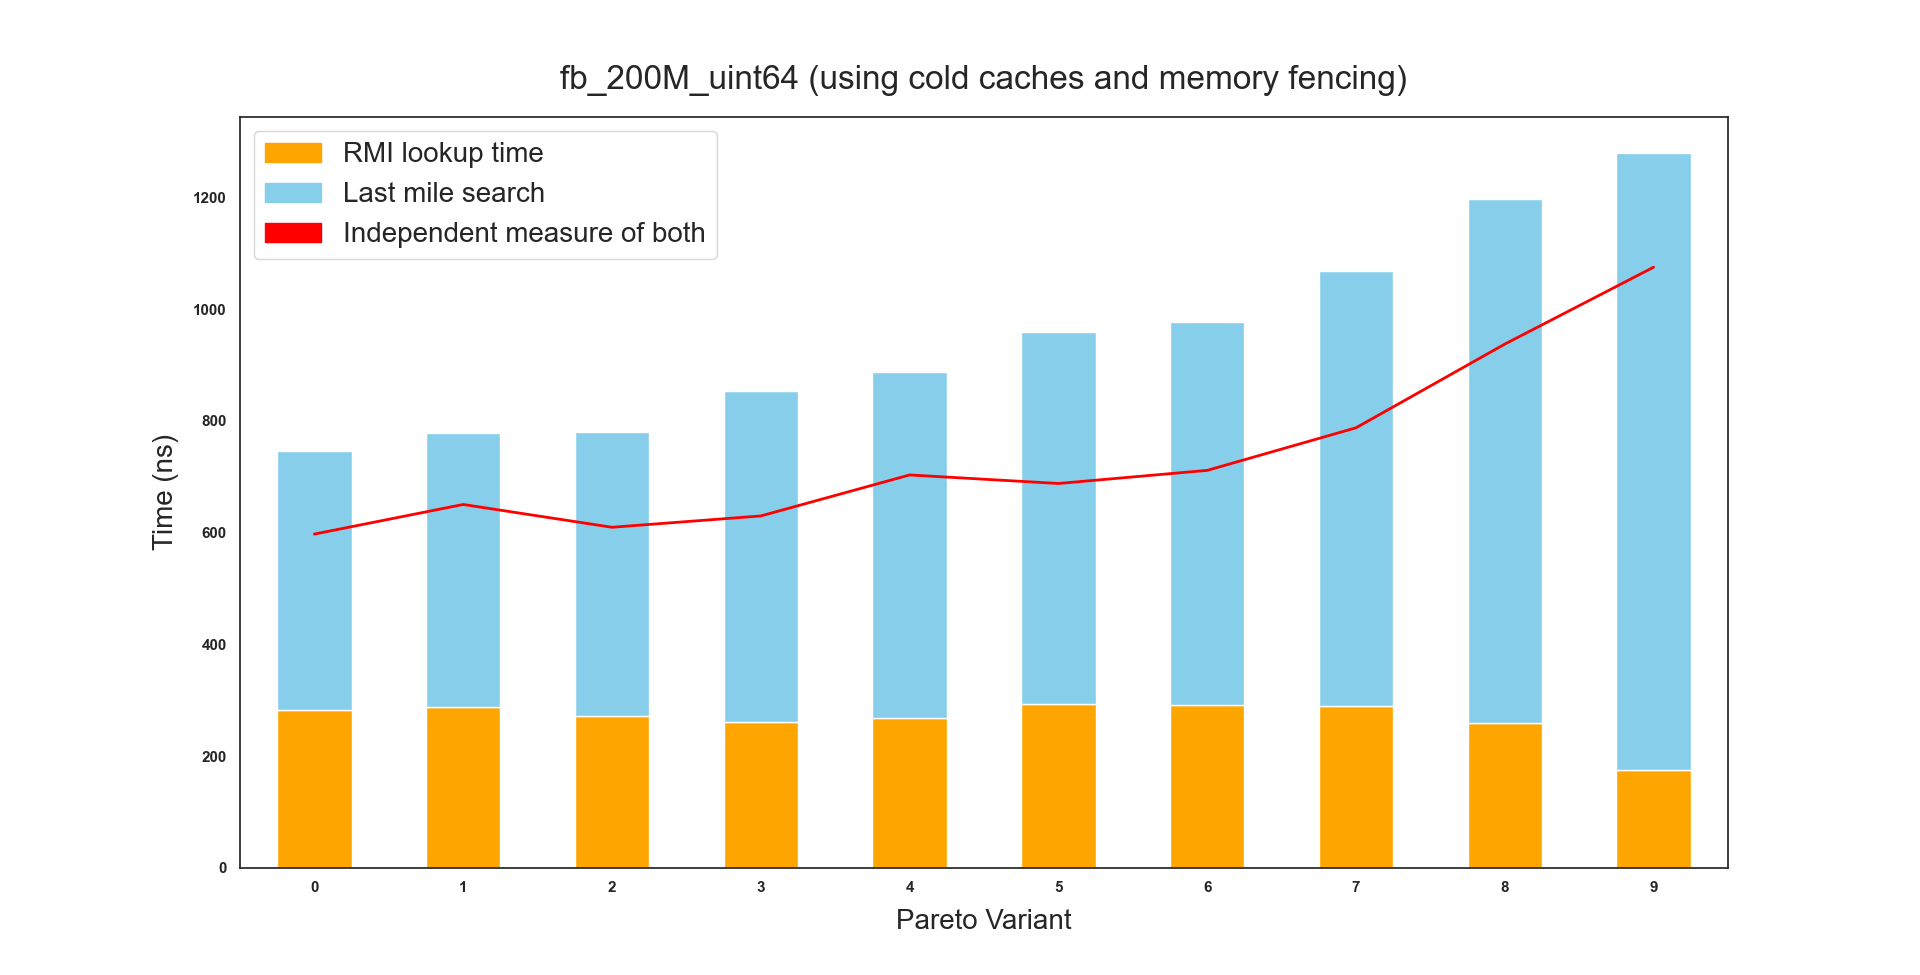
\includegraphics[width=1\textwidth]{measurements/fb_200M_uint64}
  \caption*{
    Running the SOSD benchmark on the \emph{fb\_200M\_uint64} dataset \emph{using} cold caches and memory fencing, differentiating between pure lookup time and last mile search time.
  }
\end{figure}

\begin{figure}[!htb]
  \centering
  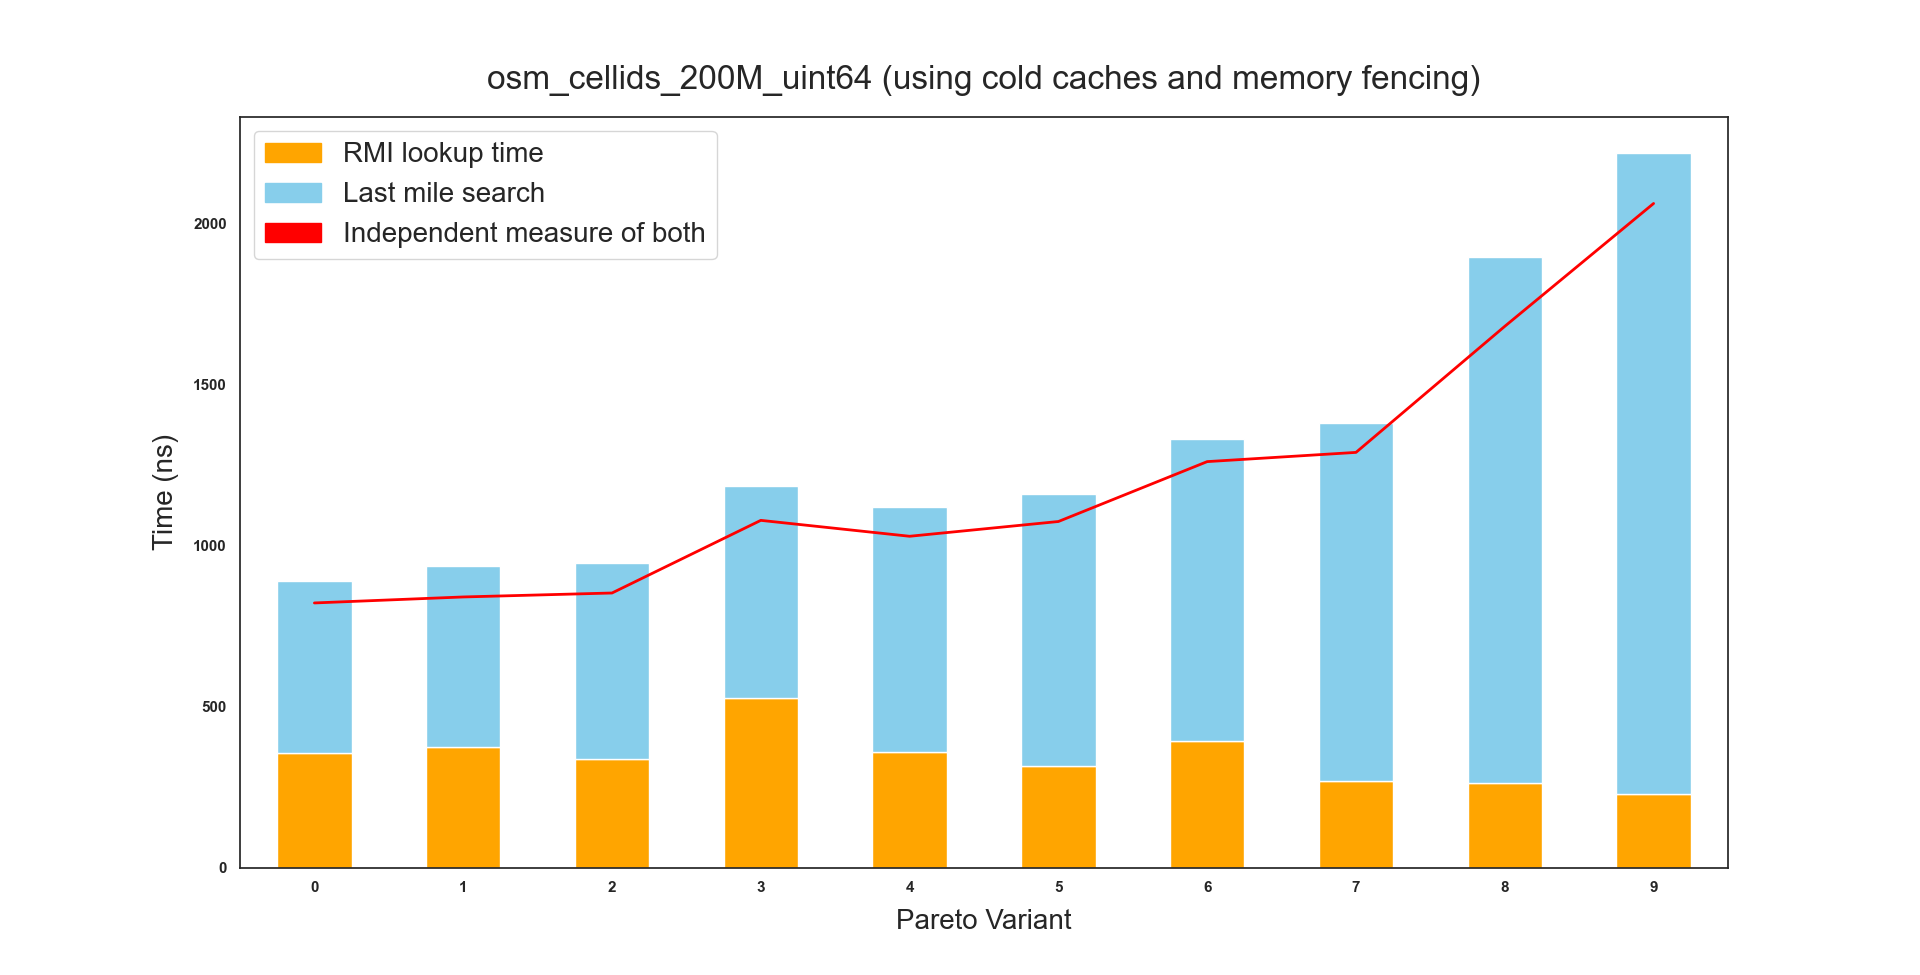
\includegraphics[width=1\textwidth]{measurements/osm_cellids_200M_uint64}
  \caption*{
    Running the SOSD benchmark on the \emph{osm\_cellids\_200M\_uint64} dataset \emph{using} cold caches and memory fencing, differentiating between pure lookup time and last mile search time.
  }
\end{figure}

\begin{figure}[!htb]
  \centering
  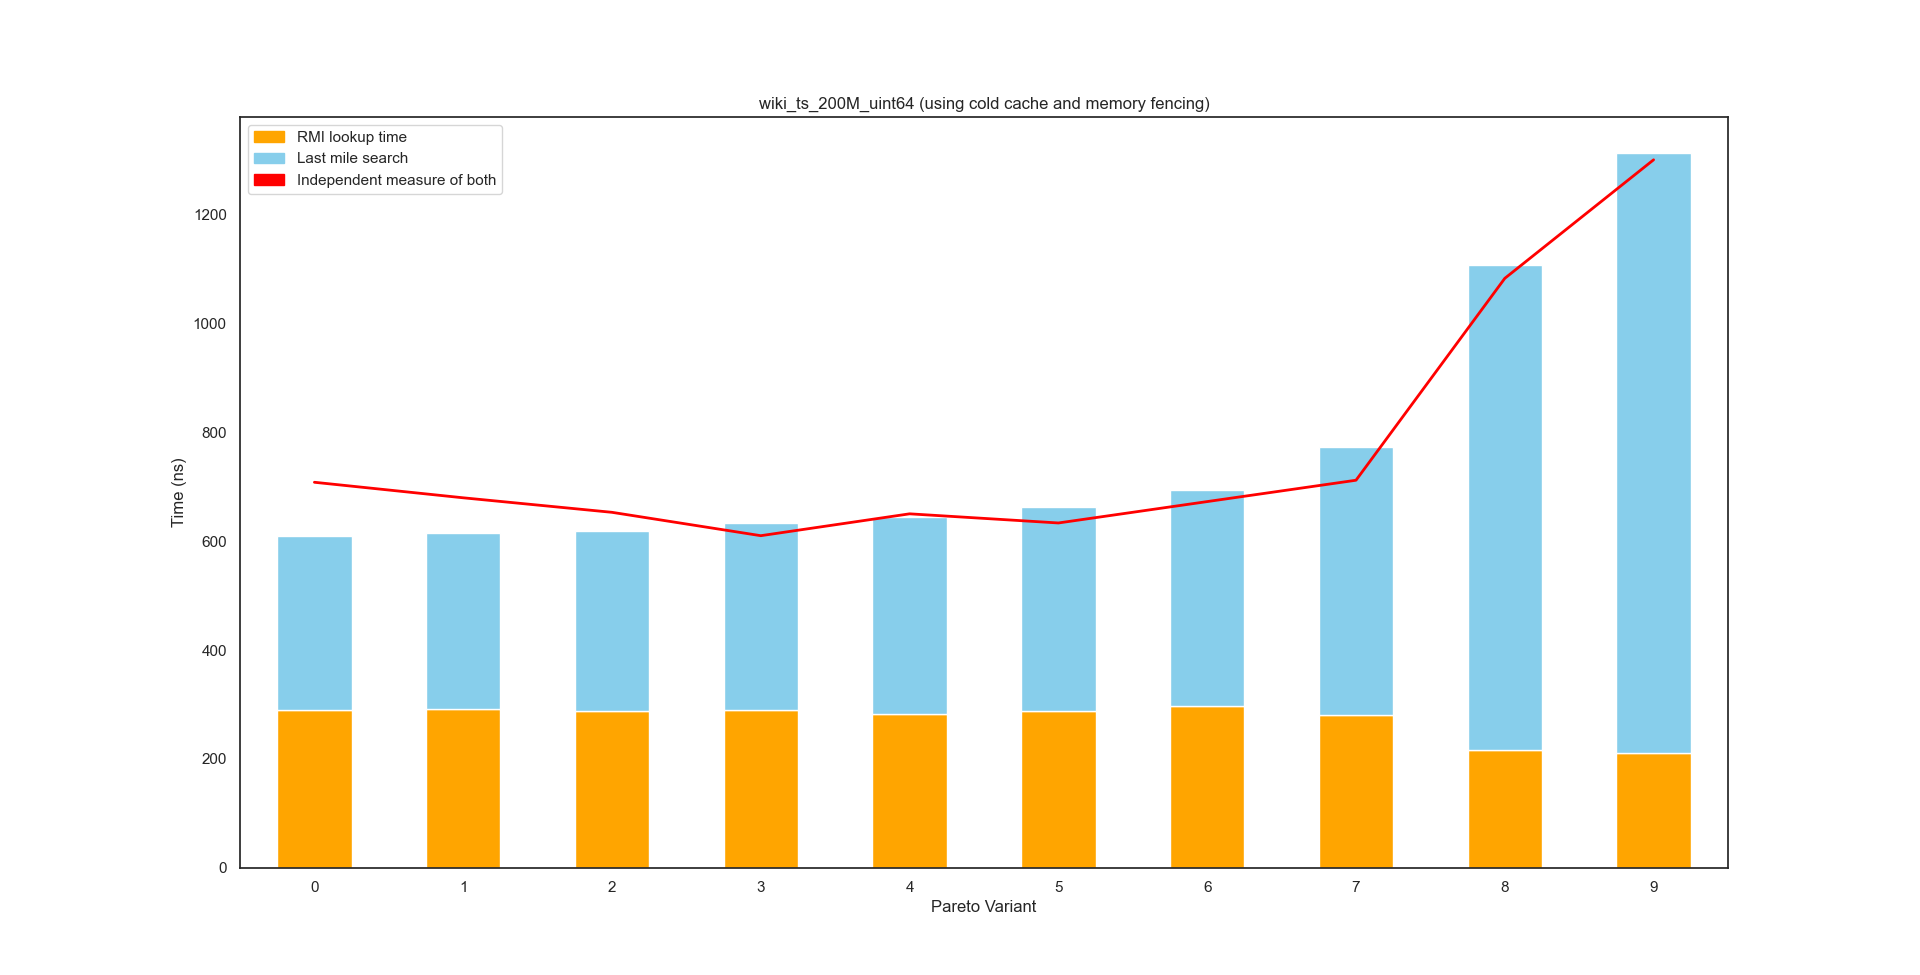
\includegraphics[width=1\textwidth]{measurements/wiki_ts_200M_uint64}
  \caption*{
    Running the SOSD benchmark on the \emph{wiki\_ts\_200M\_uint64} dataset \emph{using} cold caches and memory fencing, differentiating between pure lookup time and last mile search time.
  }
\end{figure}

\newpage % ugly, but otherwise latex does not place section title correctly

\section{Experiment results calculating pure lookup time as the difference of the total time measured and last mile search time}
\label{sect:appendix:measurements-no-lookup}

\captionsetup[figure]{skip=10pt} % move caption down
\begin{figure}[!htb]
  \centering
  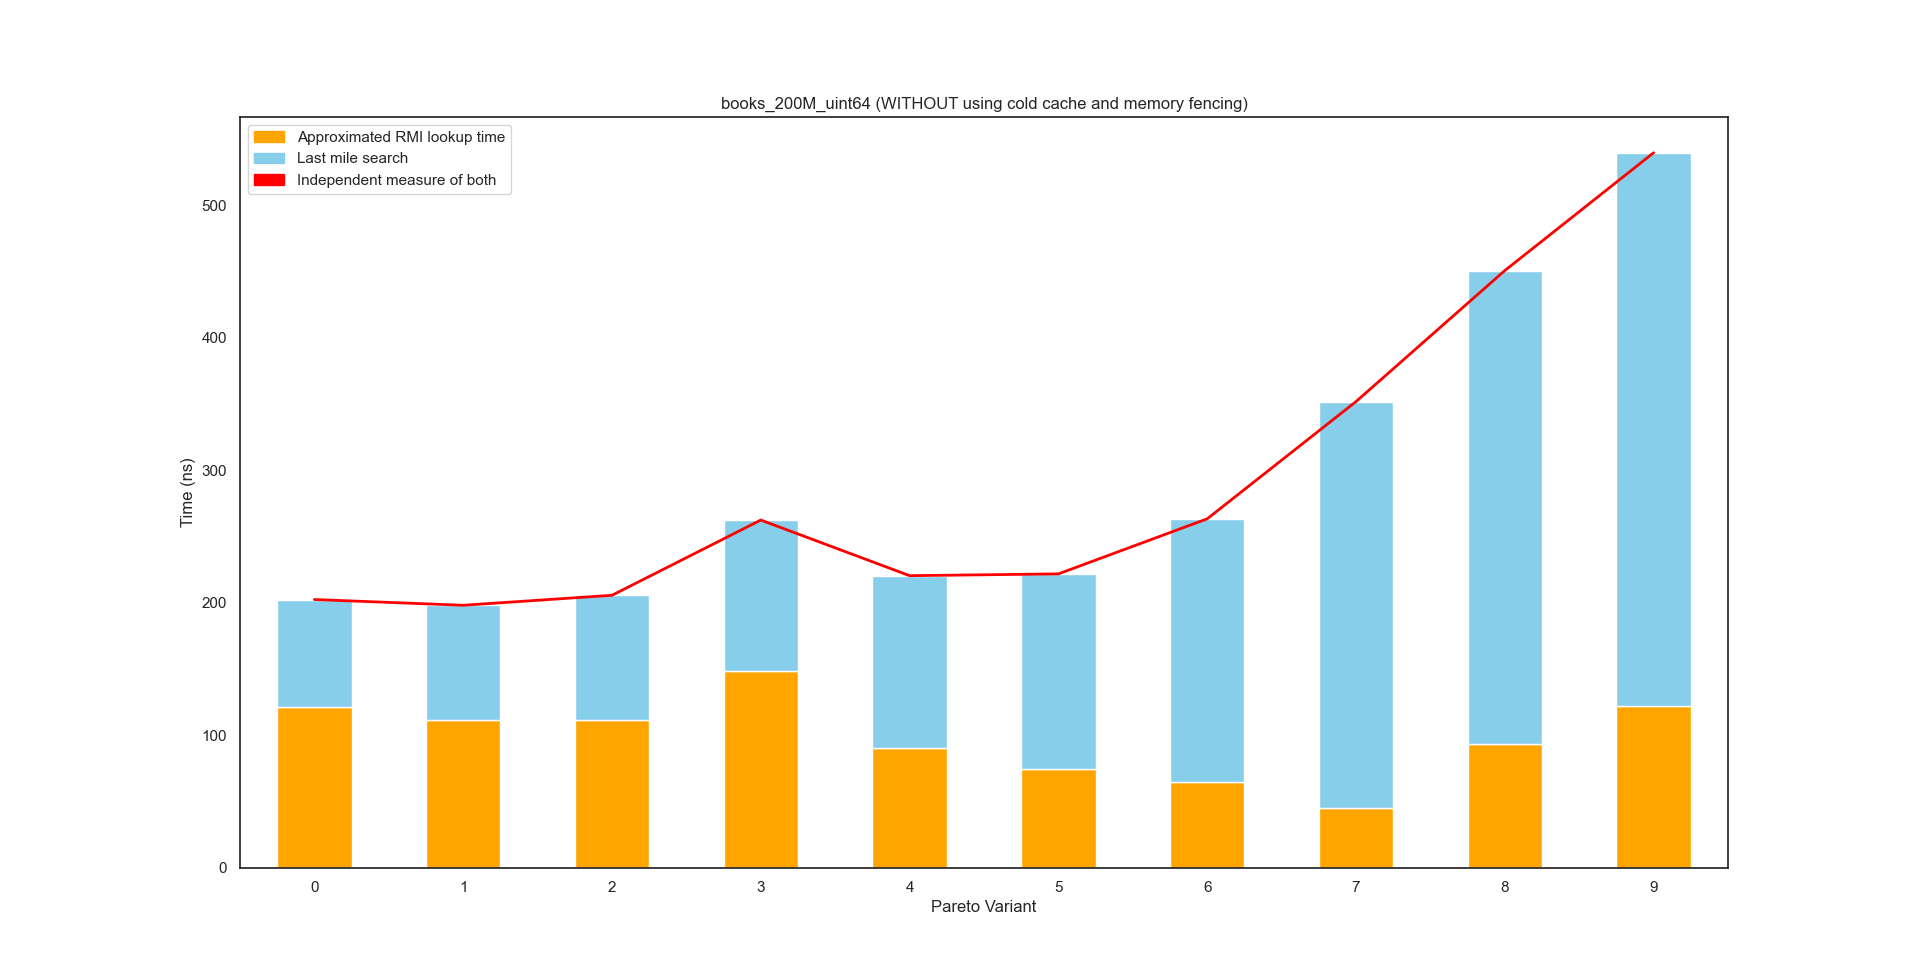
\includegraphics[width=1\textwidth]{measurements/books_200M_uint64-no-lookup}
  \caption*{
    Running the SOSD benchmark on the \emph{books\_200M\_uint64} dataset \emph{without using} cold caches and memory fencing, trying to approximate pure lookup time by subtracting last mile search time from the totally measured time.
  }
\end{figure}

\begin{figure}[!htb]
  \centering
  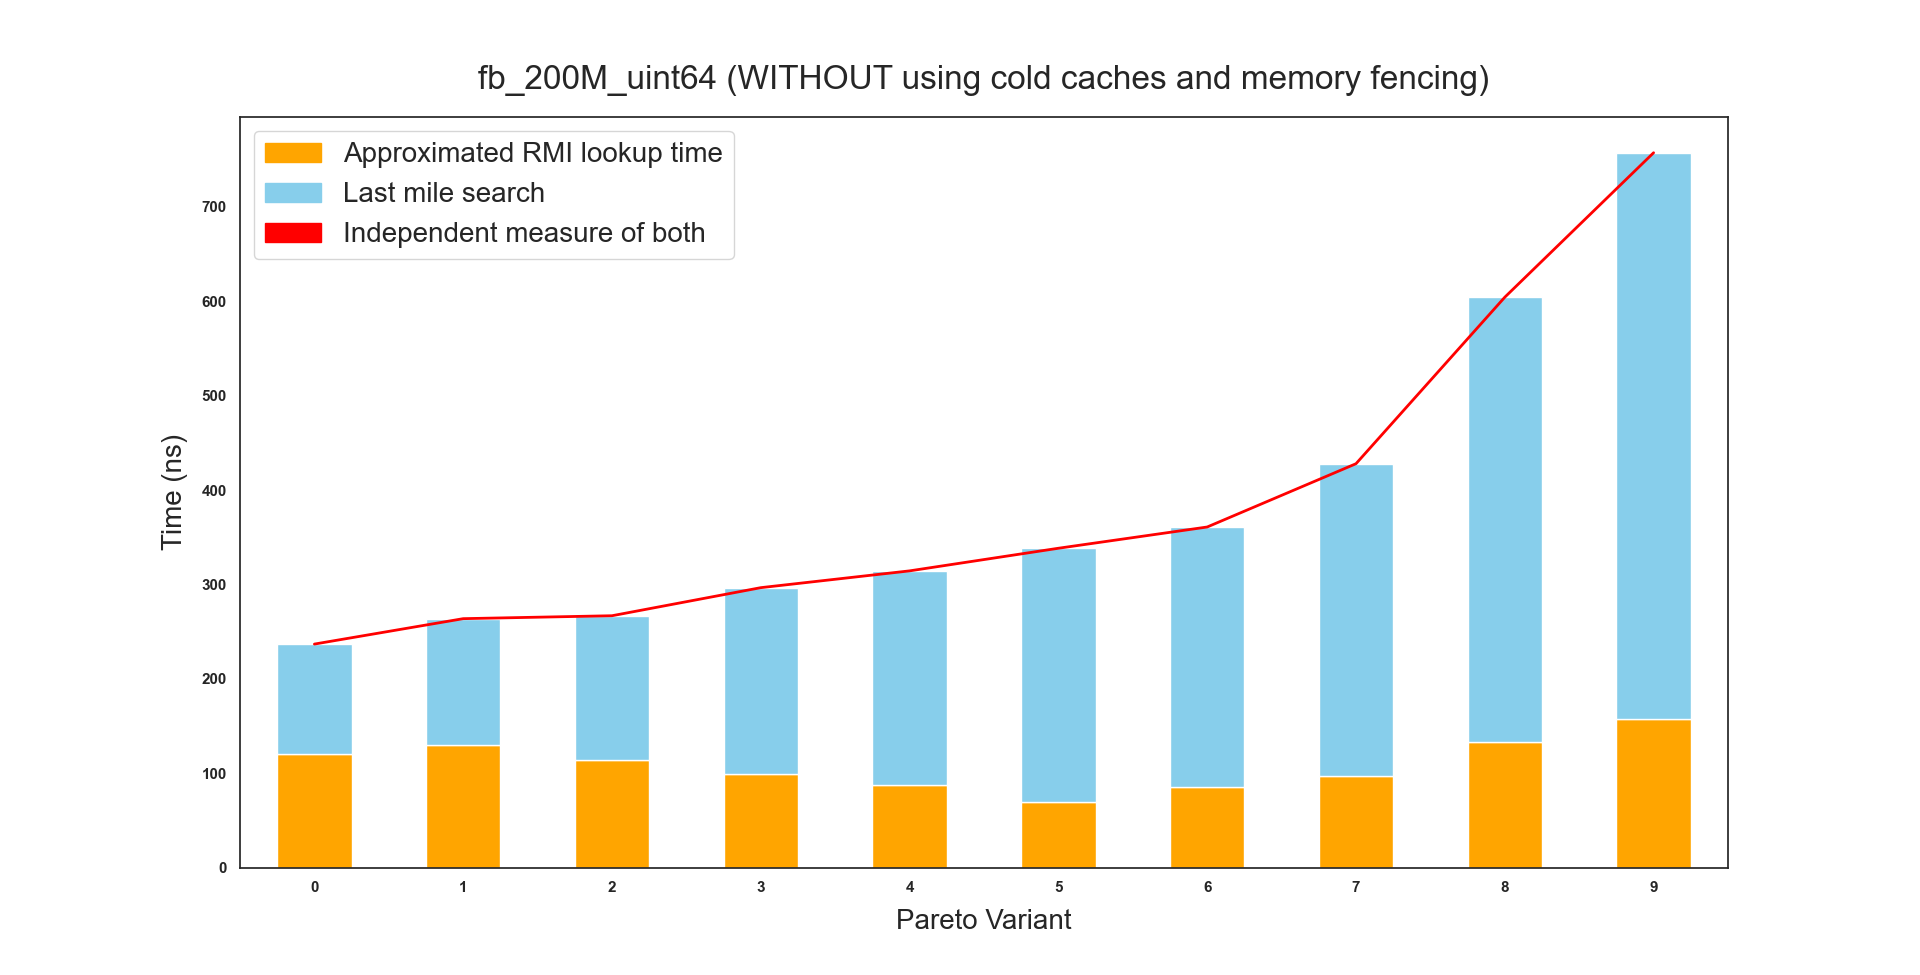
\includegraphics[width=1\textwidth]{measurements/fb_200M_uint64-no-lookup}
  \caption*{
    Running the SOSD benchmark on the \emph{fb\_200M\_uint64} dataset \emph{without using} cold caches and memory fencing, trying to approximate pure lookup time by subtracting last mile search time from the totally measured time.
  }
\end{figure}

\begin{figure}[!htb]
  \centering
  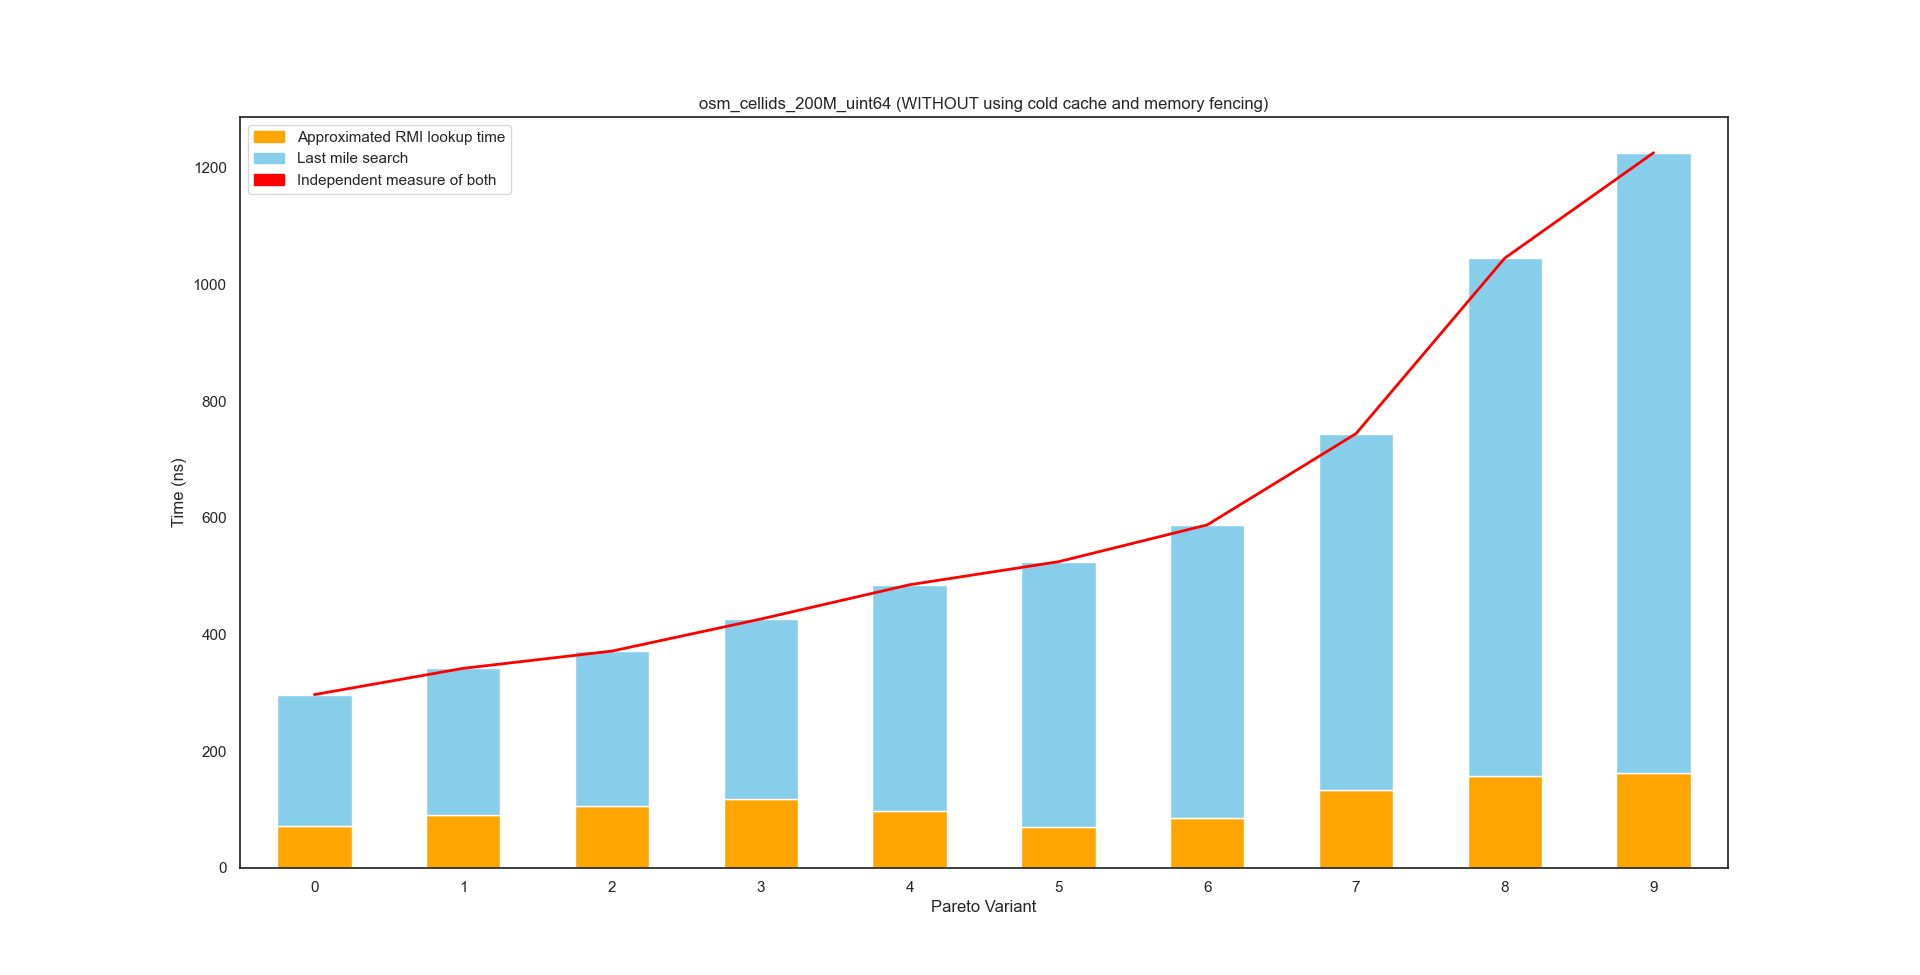
\includegraphics[width=1\textwidth]{measurements/osm_cellids_200M_uint64-no-lookup}
  \caption*{
    Running the SOSD benchmark on the \emph{osm\_cellids\_200M\_uint64} dataset \emph{without using} cold caches and memory, fencing trying to approximate pure lookup time by subtracting last mile search time.
  }
\end{figure}

\begin{figure}[!htb]
  \centering
  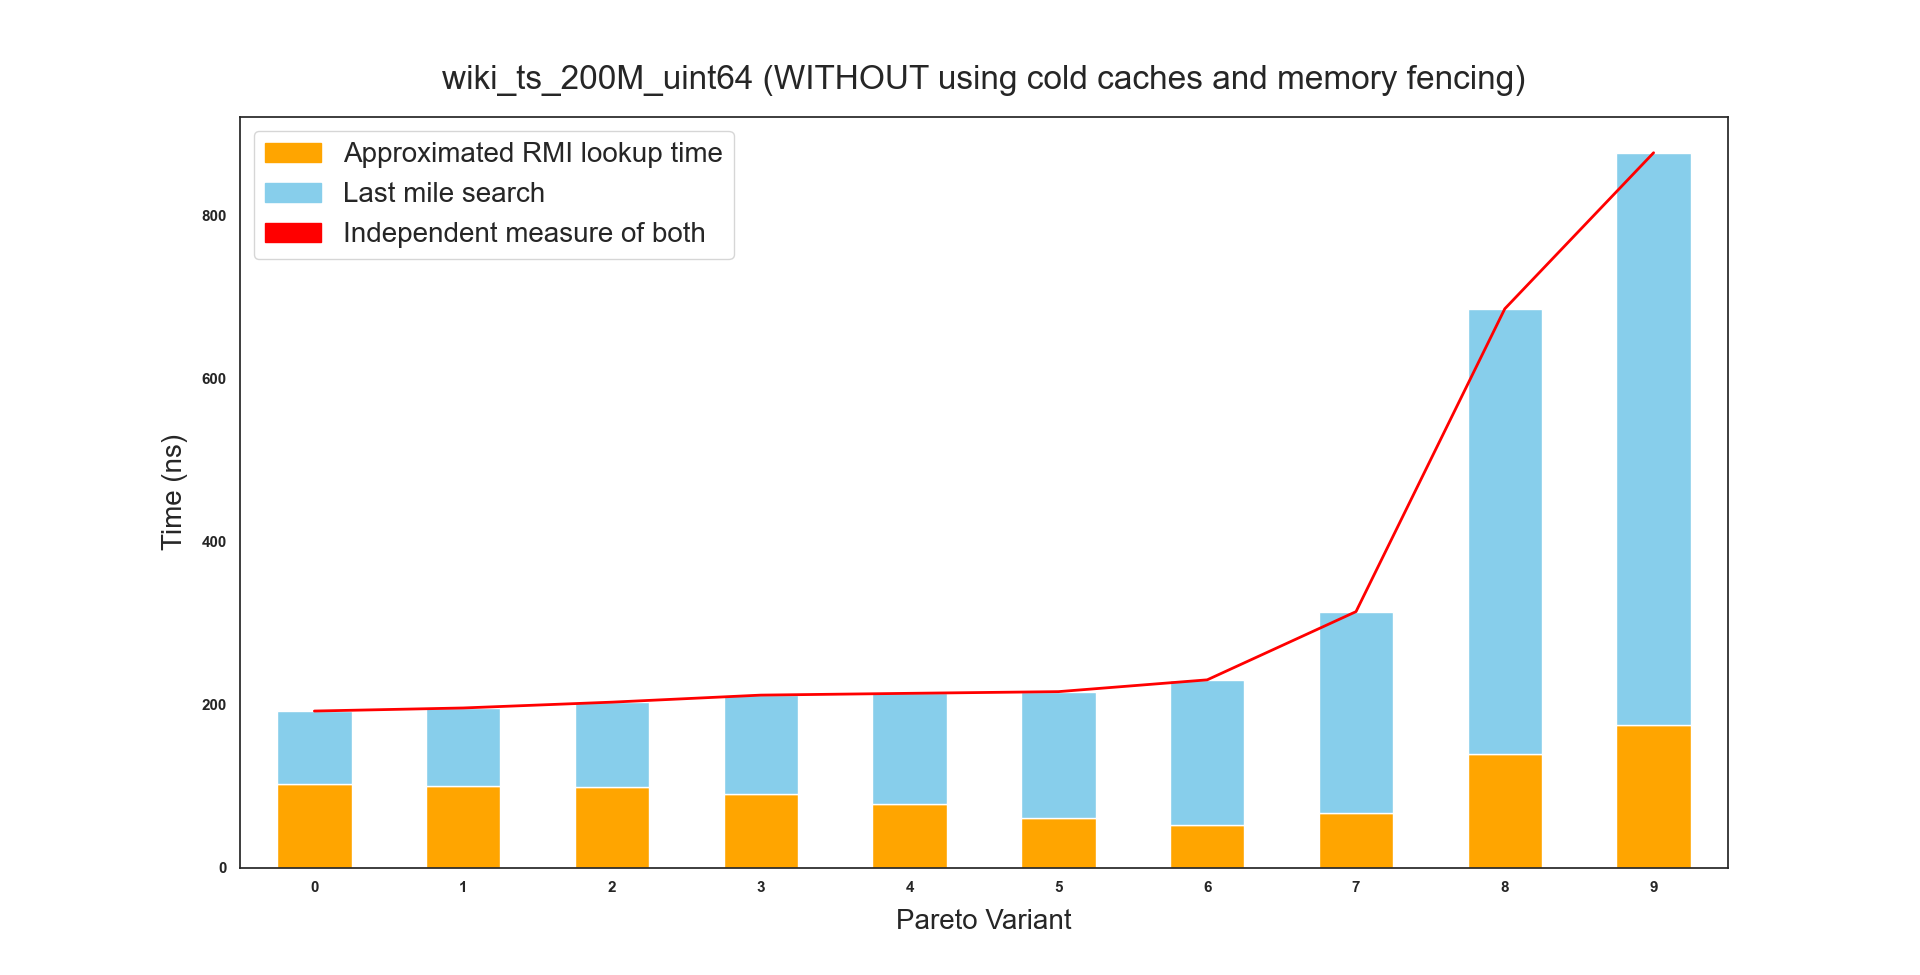
\includegraphics[width=1\textwidth]{measurements/wiki_ts_200M_uint64-no-lookup}
  \caption*{
    Running the SOSD benchmark on the \emph{wiki\_ts\_200M\_uint64} dataset \emph{without using} cold caches and memory fencing, trying to approximate pure lookup time by subtracting last mile search time from the totally measured time.
  }
\end{figure}
